%+----------------------------------------------------------------------------+
%| SLIDES: PostDoc interview - CTU
%|                https://euraxess.ec.europa.eu/jobs/612030
%| Contents: 4 slides
%|					 (extimated duration 1.5 minutes per slide )
%| Author: Antonio miti
%| Place: Amandola, Giugno 2021
%+----------------------------------------------------------------------------+


%- HandOut Flag -----------------------------------------------------------------------------------------
\newif\ifHandout
	\Handouttrue  %uncomment for the printable version


%- D0cum3nt ----------------------------------------------------------------------------------------------
\ifHandout
	\documentclass[handout,10pt]{beamer}   
	\setbeameroption{show notes} %print notes   
\else
	\documentclass[10pt]{beamer}
\fi


%- Packages ----------------------------------------------------------------------------------------------
\usepackage{custom-style}

\usetikzlibrary{backgrounds}
  \tikzset{
    invisible/.style={opacity=0},
    visible on/.style={alt=#1{}{invisible}},
    alt/.code args={<#1>#2#3}{%
      \alt<#1>{\pgfkeysalso{#2}}{\pgfkeysalso{#3}} % \pgfkeysalso doesn't change the path
    },
  }

%--Beamer Style-----------------------------------------------------------------------------------------------
\usetheme{toninus}

\usepackage{textpos,eso-pic}
\usepackage{fontawesome}



\AtBeginSubsection[]{}









%---------------------------------------------------------------------------------------------------------------------------------------------------
%- D0cum3nt -----------------------------------------------------------------------------------------------------------------------------------
\begin{document}
%---------------------------------------------------------------------------------------------------------------------------------------------------

%---------------------------------------------------------------------------------------------------------------------------------------------------
\begin{frame}{About the PostDoc Position at CTU}
\textbf{My profile}
\vspace{1em}
\begin{itemize}
	\item[•] Master degree in Physics \\ 
	\small \qquad(focus on \emph{geometric mechanics} and \emph{algebraic quantum field theory}).
	\item[•] Phd in Mathematics \\
	\small \qquad (focus on \emph{multisymplectic geometry} and \emph{algebraic methods in differential geometry}).	
\end{itemize}

\pause
\vfill
\textbf{Expertise required}
\vspace{1em}
\begin{itemize}
	\setlength\itemsep{1em}
	\item superintegrability in classical and quantum mechanics;
	\item\alert<3->{Lie groups/algebras and applications to symmetries in mathematical physics.}
\end{itemize}
\vfill
\end{frame}
%---------------------------------------------------------------------------------------------------------------------------------------------------

%---------------------------------------------------------------------------------------------------------------------------------------------------
\begin{frame}[fragile]{Recent Research Focus}
\tikzstyle{every picture}+=[remember picture]
	
	\begin{center}
		\large
		 \tikz[baseline]{
		            \node[fill=orange!20,anchor=base] (t1)
		            {Hamiltonian actions};
			}
		on
		 \tikz[baseline]{
	            \node[fill=green!20,anchor=base] (t2)
	            {multisymplectic manifolds};
		}
	\end{center}

	\begin{columns}
    	\begin{column}{.45\textwidth}
 		 \tikz[baseline]{
	            \node[visible on=<3->,draw=orange!80,anchor=base,text width=5.5cm] (s1)
	            {
						\begin{itemize}
							\item[•] Lie algebra action admitting a certain $L_\infty$-algebra lift.
							\item[•] The lift is called \emph{Homotopy comomentum map}.
							\item[•] Elements of the image can be interpreted as \emph{conserved quantities}.
						\end{itemize}
	            };
		}		   	
		\end{column}
    	\begin{column}{.45\textwidth}
		\tikz[baseline]{
	            \node[visible on=<2->,draw=green!80,anchor=base,text width=5.5cm] (s2)
	            {
						\begin{itemize}
							\item[•] Higher analogue of symplectic manifolds ($k$-forms instead of $2$-forms).
							\item[•] Inspired by the geometric formulation of classical field theories.
						\end{itemize}							            
	            };
		}	
		\end{column}
	\end{columns}



	\begin{tikzpicture}[overlay]
        \path[visible on=<3->,->,orange!80] (s1) edge [bend left] (t1);
	     \path[visible on=<2->,->,green!80] (s2) edge [bend right] (t2);
	\end{tikzpicture}

	\vfill
%	\onslide<4->{
%		\begin{center}
%			\large
%			\bf
%			Framework: \alert{\emph{Geometric Mechanics}}
%		\end{center}
%	}
\end{frame}
%---------------------------------------------------------------------------------------------------------------------------------------------------


%-------------------------------------------------------------------------------------------------------------------------------------------------
	\begin{frame}{Results}
		\vspace{1em}
		
		\begin{columns}
			\begin{column}[T]{0.3\textwidth}
				\centering
				\onslide<1->{
					\fbox{
\includegraphics[width=.9\textwidth]{../Pictures/cover-JAMS}}
				}
			\end{column}		
			\begin{column}[T]{0.7\textwidth}
				\begin{itemize}
					\item[-] Explicit \emph{Homotopy comomentum map} coming from hydrodynamics ( ideal fluid configurations as Lie algebra action)
					\item[-] Relations with \emph{knot theory} (hydrodinamics interpretation: links as concentrated vortices).
				\end{itemize}
			\end{column}		
		\end{columns}	
		
		\vspace{1em}
		\begin{columns}[T]
			\begin{column}{0.3\textwidth}
				\centering
				\onslide<2->{
					\fbox{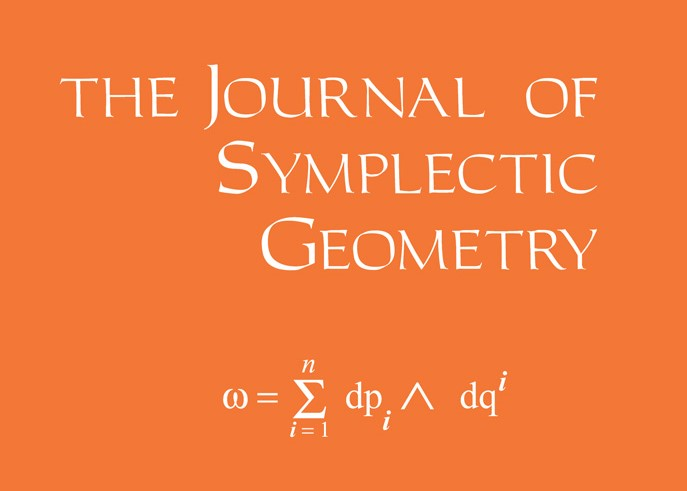
\includegraphics[width=.9\textwidth]{../Pictures/cover-JSG}}
				}
			\end{column}		
			\begin{column}{0.7\textwidth}
				\begin{itemize}
					\item<2->[-] Complete classification of Hamiltonian actions on spheres (multisymplectic w.r.t. the canonical volume form.
					\item<2->[-] Explicit expression of momenta for $SO(n)\circlearrowleft S^n$ and other cases.
				\end{itemize}
			\end{column}		
		\end{columns}		
		
		\vspace{1em}
		\begin{columns}[T]
			\begin{column}{0.3\textwidth}
				\centering
				\onslide<3->{
					\fbox{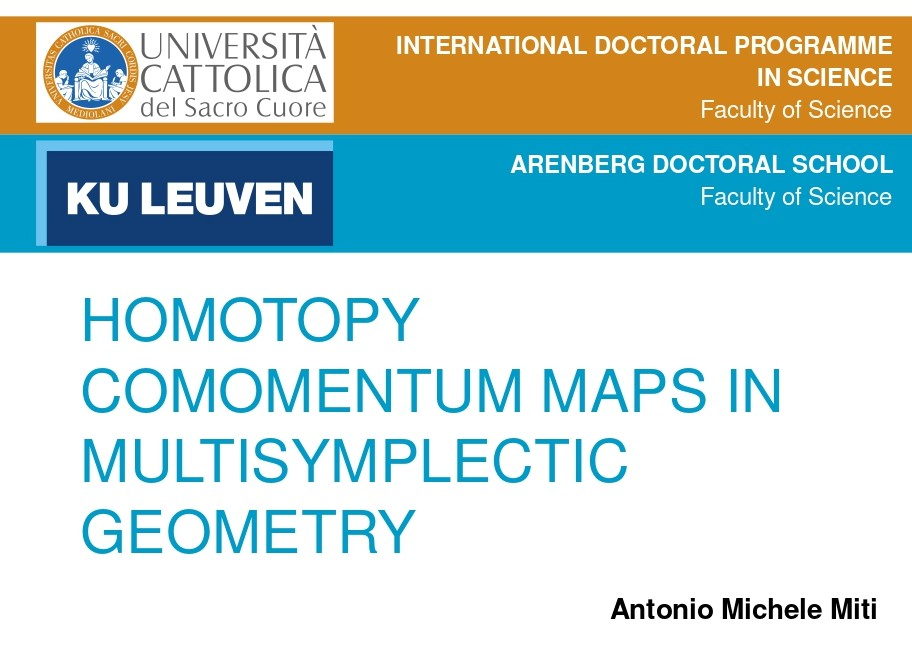
\includegraphics[width=.9\textwidth]{../Pictures/cover-Thesis}}
				}
			\end{column}		
			\begin{column}{0.7\textwidth}
				\begin{itemize}
					\item<3->[-] Compatibility of \emph{Homotopy comomentum maps} w.r.t. gauge-related multisymplectic manifolds.
					\item<3->[-] Relationship between the $L_\infty$-algebra of observables and \emph{higher courant algebroids.} 				\end{itemize}	
			\end{column}		
		\end{columns}
		\vfill
\end{frame}
%---------------------------------------------------------------------------------------------------------------------------------------------------


%%-------------------------------------------------------------------------------------------------------------------------------------------------
%	\begin{frame}{Skills transferable outside of the multisymplectic geometry context }
%		\begin{itemize}
%			\item Expertise in explicit constructions/computations involved homotopy structures
%			\begin{itemize}
%				\item borrowing tools from the context of \emph{deformation theory}.
%				\item eventually computer-aided (via symbolic calculus).
%			\end{itemize}
%			\item Translation of field theoretic construction from the covariant phase framework (infinite dimensional) to the multisymplectic one.
%		\end{itemize}
%
%	\end{frame}
%-------------------------------------------------------------------------------------------------------------------------------------------------









%------------------------------------------------------------------------------------------------
% APPENDIX
%------------------------------------------------------------------------------------------------
\appendix
\part{EXTRA}
%\sectionpage
\begin{frame}
	\begin{center}
	\Huge\emph{Backup Slides}
	\end{center}
\end{frame}
\addtocounter{framenumber}{-1}


%-------------------------------------------------------------------------------------------------------------------------------------------------
\section{Background}
%\checkpoint
%-------------------------------------------------------------------------------------------------------------------------------------------------
%-------------------------------------------------------------------------------------------------------------------------------------------------
\subsection{Multisymplectic geometry}
%-------------------------------------------------------------------------------------------------------------------------------------------------



%-------------------------------------------------------------------------------------------------------------------------------------------------
\begin{frame}[fragile]{Multisymplectic manifolds} %Fragile -->workaround tikzcd
	\begin{defblock}[$n$-plectic manifold ~\emph{(Cantrijn, Ibort, De Le\'on)}]
	\includestandalone[width=0.95\textwidth]{../Pictures/Figure_multisym}	
	\end{defblock}
	%
	\begin{defblock}[Non-degenerate $(n+1)$-form]
		\begin{columns}
			\begin{column}{.45\linewidth}
				\centering{
				The $\omega^\flat$ (flat) bundle map is injective.
				}
			\end{column}
			\begin{column}{.5\linewidth}
						\vspace{-.5em}
				\[
				\begin{tikzcd}[column sep= small,row sep=0ex,
				/tikz/column 1/.append style={anchor=base east}]
				    \omega^\flat \colon T M \ar[r]& \Lambda^n T^\ast M \\
  						 (x,u) \ar[r, mapsto]& (x,\iota_{u} \omega_x)						
				\end{tikzcd}	
				\]
			\end{column}
		\end{columns}
	\end{defblock}
	%
	\pause
	\begin{defblock}[Hamiltonian $(n-1)$-forms]
		\begin{displaymath}
			\Omega^{n-1}_{ham}(M,\omega) 	:=
			\biggr\{ \sigma \in  \Omega^{n-1}(M) \; \biggr\vert \; 
				\exists \mathscr{v}_\sigma \in \mathfrak{X}(M) ~:~ 
				\tikz[baseline,remember picture]{\node[rounded corners,
                        fill=orange!10,draw=orange!30,anchor=base]            
            			(target) {$d \sigma = -\iota_{\mathscr{v}_\sigma} \omega$ };
            	}				
				~\biggr\} 
			\end{displaymath}
	\end{defblock}
	%
	%
	\pause
		\tikz[overlay,remember picture]
		{
			\node[rounded corners,
                 fill=orange!10,draw=orange!30,anchor=base]            
            	 (base) at ($(current page.east)-(2.25,1.8)$) [rotate=-0,text width=4cm,align=center] {\small\textcolor{red}{Hamilton-DeDonder-Weyl \\equation}};
		}	
	\begin{tikzpicture}[overlay,remember picture]
    	\path[->] (base.west) edge[bend left,red](target.south west);
    \end{tikzpicture}	
	\pause
	\vfill
	%
	\begin{block}{Examples:}
		\vspace{-.5em}
		\setbeamercovered{transparent}
		\begin{itemize}[<+->]
			\item[$\bullet$] $n=1$ \qquad\qquad\qquad $\Rightarrow$\quad $\omega$ is a symplectic form
			\item[$\bullet$]  $n=(dim(M)-1)$ \quad$\Rightarrow$\quad $\omega$ is a volume form
			%Any oriented $(n+1)$-dimensional manifold is $n$-plectic w.r.t. the volume form.
			%\item[$\bullet$] Let $G$ a semisimple Lie group and $\langle\cdot,\cdot \rangle$  its killing form. Then $\langle [\cdot,\cdot],\cdot \rangle$ extends to a biinvariant multisymplectic form $\omega$.
			\item[$\bullet$] Let $Q$ a smooth manifold, the multicotangent bundle $\Lambda^n T^\ast Q$ is naturally $n$-plectic.%
			\quad
			\textit{(cfr, \href{https://arxiv.org/abs/physics/9801019}{GIMMSY} construction for classical field theories)}
		\end{itemize}
	\end{block}			 
	
%
\end{frame}
\note[itemize]{
	\item Multisymplectic ($n$-plectic) geometry is a generalization of symplectic geometry where a closed, non degenerate $n+1$-form $(n\geq 1)$  takes the place of the symplectic 2-form
	
	\item multisymplectic means \emph{going higher} in the degree of $\omega$
	
	\item non degeneracy means $\iota_v\omega = 0 \Leftrightarrow v=0$.
	
	\item examples 
		\begin{itemize}
			\item[$\bullet$] 1-plectic $=$ symplectic
			\item[$\bullet$] Any oriented $(n+1)$-dimensional manifold is $n$-plectic w.r.t. the volume form.
			\item[$\bullet$] The multicotangent bundle $\Lambda^n T^\ast Q$ is naturally $n$-plectic.
		\end{itemize}
	
	\item We recognize the special class of forms, called Hamiltonian, determining the Hamiltonian vector fields. 
	Not every $n-1$ form admits an Hamiltonian vector field.
	When it exists, non degeneracy guarantees unicity.
	
	\item Observe also that, by degree reason, when $n$ is equal to $1$ or $dim(M)+1$ an injective flat map $\flat$ is also bijective.
	
	\item It is important to stress that mechanical systems are not the only source instances of this class of of structures. 
				e.g. any semisimple Lie groups has associated a 2-plectic structure and any oriented $n+1$ dimensional manifold is naturally $n$-plectic.
				

}
%---------------------------------------------------------------------------------------------------------------------------------------------------








%---------------------------------------------------------------------------------------------------------------------------------------------------
\subsection{Lie $\infty$-algebra of Observables}
%-------------------------------------------------------------------------------------------------------------------------------------------------
\begin{frame}[fragile,t]{Lie $\infty$-algebra of Observables (higher observables) }
	Let be $(M,\omega)$ a $n$-plectic manifold.
	\begin{defblock}[$L_\infty$-algebra of observables ~\emph{(Rogers)}]
		\hspace{.25em} Is a co-chain complex $(L,\{\cdot\}_1)$ \\
		\vspace{-2.5em}
		\begin{center}
		\ifHandout
			\includestandalone{../Pictures/Figure_Observables}	
		\else
			\includestandalone{../Pictures/Frame_Observables}
		\fi				
		\end{center}
		\onslide<2->{
			\hspace{.25em} with $n$ (skew-symmetric) multibrackets $(2 \leq k \leq n+1)$\\
			\vspace{-1.5em}
			\begin{center}
				\includestandalone{../Pictures/Equation_Multibracket}	
			\end{center}
		}
		%
	\end{defblock}
  	\vfill
	\onslide<3->{
		\emph{Higher analogue} of the \emph{Poisson algebra structure} associated to a symplectic mfd.
	\vfill
	\begin{columns}
		\hfill
		\begin{column}{.11\linewidth}	
			If $n>1$:
			
		\end{column}	
		\begin{column}{.8\linewidth}
		\begin{itemize}
			\item[\xmark] \textcolor{red}{we lose} :\quad multiplication of observables, Jacobi equation;
			%\\ \hspace*{4.25em} full-fledged Jacobi equation;
			\item[\cmark] \textcolor{green}{we gain} :\quad brackets with arities different than two,\\
			\hspace*{4.25em}
			 Jacobi equation \emph{up to homotopies}.
		\end{itemize}		
		\end{column}		
	\end{columns}
	}
  \end{frame}
 \note[itemize]{
	\item if symplectic manifolds are the symmetric take on mechanics, Poisson algebras are the algebraic counterpart.
 	\item A Lie algebra is associated to an ordinary symplectic manifold (its Poisson algebra).
	%(Underlying this is a Lie algebra, whose Lie bracket is the Poisson bracket.)
	Similarly, one associates an Lie-$n$ algebra to any $n$-plectic manifold.
 	% https://ncatlab.org/nlab/show/n-plectic+geometry 	 
 	 %https://ncatlab.org/nlab/show/Poisson+bracket+Lie+n-algebra
	 \item Basically, the higher observables algebra is a chunk of the de Rham complex of $M$ with inverted grading( convention employed here) and an extra structure called "multibrackets".
 	\item ( In the 1-plectic case it reduces to the corresponding Poisson algebra of classical observables)
 	\item Rogers associated to any n-plectic mfd a $L\-\infty$ algebra, Zambon generalized it to the pre-n-plectic case.
 	\item Recognize in the definition of $\{\cdot,\ldots,\cdot\}_k$ the contraction with hamiltonian fields $v_\sigma$ w.r.t. $\sigma$.
  	\item Note $	\iota_{v_{\sigma_1}}\cdots\iota_{v_{\sigma_k}} = (-)^{(k-1)+(k-2)+\dots+1}\iota_{v_{\sigma_k}}\cdots\iota_{v_{\sigma_1}} = (-)^{\frac{k(k-1)}{2}}\iota_{v_{\sigma_k}}\cdots\iota_{v_{\sigma_1}}$ 
 	The definition usually find in literature of Rogers multibrackets involves the coefficient $ (-)^{\frac{k(k-1)}{2}} = -\varsigma(k-1) = (-)^{k+1} \varsigma(k)$.
  \item higher observables is Special instance of a more general object  called $L\-\infty$ Algebra...
 }
%------------------------------------------------------------------------------------------------


%-------------------------------------------------------------------------------------------------------------------------------------------------
\subsection{Homotopy comomentum maps}
%-------------------------------------------------------------------------------------------------------------------------------------------------
\begin{frame}[fragile]{Homotopy comomentum maps}
	Consider a Lie algebra action $v:\mathfrak{g} \to \mathfrak{X}(M)$  \underline{preserving the $n$-plectic form $\omega$}.
	\vfill
	\begin{defblock}[Homotopy comomentum map \emph{(Callies, Fregier, Rogers, Zambon)}]
		\ifHandout
			\includestandalone{../Pictures/Figure_Lifting}
		\else
			\includestandalone{../Pictures/Frame_Lifting}
		\fi					
	\end{defblock}
	\vfill
	\onslide<4->{
	\begin{lemblock}[HCMM unfolded  \cite{Callies2016}]
			%
			HCMM is a sequence of (graded-skew) multilinear maps:
			\begin{displaymath}
				(f)  = \big\lbrace f_k: \; \Lambda^k{\mathfrak g} \to L^{1-k} \subseteq \Omega^{n-k}(M) 
				~\big\vert~ 0\leq k \leq n+1  \big\rbrace
			\end{displaymath}
			\emph{fulfilling:}%\emph{such that:}
			\begin{itemize}
				\item<5-> $f_0 = 0 $, $f_{n+1} = 0$
				\item<6-> $d f_k (p) = f_{k-1} (\partial p)  - (-1)^{\frac{k(k+1)}{2}} \iota(v_p) \omega 
				\qquad\scriptstyle \forall p \in \Lambda^k(\mathfrak{g}),\; \forall k=1,\dots n+1$
			\end{itemize}
		\end{lemblock}	
	}

\end{frame}
\note[itemize]{
	\item  An infinitesimal symmetry is a lie algebra morphism such that $\mathcal{L}_{v_x} \omega = 0 ~ \forall x \in \mathfrak{g}$.
	\\ (It is also call an infinitesimal multisymplectic action and $v_x$ is the infinitesimal generator of the action, corresponding to $x \in \mathfrak g$.) 
	\item Essentially, admitting a comoment maps mean that $v$ acts via Hamiltonian vector fields.
	\item In mechanical terms, a moment map is a tool associated with a Hamiltonian action of a Lie group on a symplectic manifold, used to construct conserved quantities for the action.(see \ref{frame:HCMMandConserved} in appendix.
}
%-------------------------------------------------------------------------------------------------------------------------------------------------





%-------------------------------------------------------------------------------------------------------------------------------------------------
\section{Foreground}
\checkpoint
%-------------------------------------------------------------------------------------------------------------------------------------------------
%-------------------------------------------------------------------------------------------------------------------------------------------------
\subsection{Applications to hydrodynamics and knot theory}
%-------------------------------------------------------------------------------------------------------------------------------------------------
\begin{frame}{Applications to hydrodynamics and knot theory (Joint with M.Spera)}
	\begin{columns}
		\begin{column}{.3\linewidth}
			$G~=~SDiff_0(\mathbb{R}^3)$
			\\
			(volume-preserving diffeomorphisms)
		\end{column}	
		\pause
		\begin{column}{.7\linewidth}
			\begin{itemize}
				\item Configuration space of an \emph{ideal fluid},
				\item (Determining) ambient isotopies of knotted links (interpreted as singular vortices)
			\end{itemize}
		\end{column}
	\end{columns}
	%
	\vfill
	\pause
	\begin{columns}
		\begin{column}{.45\linewidth}
		  	\begin{displaymath}
		  		\begin{split}
		  		&\mathfrak{g}:= sdiff_0(\mathbb{R}^3) = \\
		  		&\left\lbrace  X \in \mathfrak{X}(\mathbb{R}^3) ~\left\vert~ 
		  		\substack{ div X = 0, \\ \textrm{\emph{ rapidly vanishing at }}\infty} \right\rbrace \right.
		  		\end{split}
		  	\end{displaymath}
		\end{column}	
		\begin{column}{.55\linewidth}
			\begin{itemize}
				\item Fluid velocities
				\item Subalgebra of the  $\infty$-dim. "Lie algebra" of a $\infty$-dim "Lie group" $G$.
			\end{itemize}
		\end{column}
	\end{columns}
	\pause
	\vfill
	\begin{columns}
		\begin{column}{.3\linewidth}
			$\mathfrak{g}= sdiff_0 \hookrightarrow  \mathfrak{X}(\mathbb{R}^3)$
		\end{column}
		\begin{column}{.7\linewidth}
			\begin{itemize}
				\item Multisymplectic Lia algebra action
				\item[] w.r.t $(\mathbb{R}^3,\nu = dx\wedge dy\wedge dz)$ 2-plectic mfd.
			\end{itemize}
		\end{column}
	\end{columns}
	\pause
	\vfill
	\begin{center}
		\alert{
		\faQuestionCircle \qquad
			{Does $sdiff_0 \circlearrowleft (\mathbb{R}^3,\nu = dx\wedge dy\wedge dz)$ admit an HCMM?}	
		\qquad \faQuestionCircle		
		}
	\end{center}
	\pause
\tcbset{colback=white,
	colbacktitle=white,
	colframe=blue!70!black,
	boxrule=1pt,
	colupper=blue!70!black,
	arc=15pt,
	}
\begin{tcolorbox}[sidebyside,righthand width=.75\linewidth]
	Thm: \cite{Miti2018}
	\tcblower
	\vspace{-1.5em}
	\begin{align*}
	f_1 &= \flat \circ \text{curl}^{-1} ~:~ \mathfrak{g} \to \Omega^{1}_{Ham}(\mathbb{R}^3)
	\qquad \text{\small ("Biot-Savart law")}
	%\tag{\small"Biot-Savart law"}
	\\
	f_2 &= \Delta^{-1} \circ \delta \circ (f_1 \circ \partial_{CE} +\iota(\cdot)\omega) ~:~ \wedge^2\mathfrak{g} \to C^{\infty}(\mathbb{R}^3)
	%\tag{\small"Coulomb law"}
	\end{align*}
\end{tcolorbox}
	
	
	

	\pause
	\vfill
	Applications:
	\begin{itemize}[<+->]%[<alert@+>]
		\item[\CheckedBox]  Hydrodynamics interpretation: Rasetti-Regge currents as "momenta".
		% is exhibited upon resorting to the Euler equation for perfect fluids.
		\item[\CheckedBox]  Knot theory: reinterpretation of the (Massey) higher order linking numbers in terms of conserved quantities.
		\item[\CheckedBox]  Semiclassical interpretation of the HOMFLYPT polynomial.
	\end{itemize}

\end{frame}
\note[itemize]{
	\item relation with knot theory: looking at the knot as a fluid configuration with singular vorticity along a knotted tube,
	\item subalgebra of the infinitesimal action of $SDiff(\mathbb{R}^3)$
	\item observe how elements from Riemannian geometry and hodge theory appear in the construction
		\begin{itemize}
			\item $\delta$ codifferential
			\item $\Delta$ Laplacian
			\item $\flat$ $\sharp$  musical isomorphisms
		\end{itemize}
	\item other results of the paper: 	
	\begin{itemize}
		\item[\CheckedBox]  Explicit construction of an HCMM for $SDiff_0 \circlearrowright (\mathbb{R}^3,\nu)$ (and generalization to Riemannian homological spheres);
		\item[\CheckedBox]  Hydrodynamics interpretation: proved that this HCMM trasgresses to the standard hydrodynamical co-momentum map of  Arnol'd, Marsden and Weinstein and others;
		% is exhibited upon resorting to the Euler equation for perfect fluids.
		\item[\CheckedBox]  Application to knot theory: reinterpretation of the (Massey) higher order linking numbers in terms of conserved quantities and determined the knot theoretic analogues of first integrals in involution.
	\end{itemize}
	
}



%-------------------------------------------------------------------------------------------------------------------------------------------------



%-------------------------------------------------------------------------------------------------------------------------------------------------
\subsection{Relation to higher Courant algebroids}
%-------------------------------------------------------------------------------------------------------------------------------------------------



\begin{frame}[fragile]{Relation to higher Courant algebroids (Joint with M. Zambon)}
	%
	Consider $(M,\omega)$ \alert{symplectic mfd.}
	\only<3-11>{ and \alert{prequantizable} ($S^1$-bundle $P$, connection $\theta$)}
	\vfill
	\includestandalone[width=\textwidth]{../Pictures/Frame_BigDiagram_symplectic}
	%
	\begin{minipage}[t][2cm][t]{\textwidth}
	\begin{itemize}
		\only<1-6>{
			\item<2-> Given a Symp. mfd. $(M,\omega)$ there is a naturally associated Poisson algebra ...
			\item<4-> .\alert<+>{... and also a Lie Algebroid}.
			\item<5-> A Lie algebroid is a "controlled" $\infty$-dimensional Lie algebra;
		}
		\only<7-11>{
		\item<7-> Consider a deformed structure $\tilde{\omega}= \omega + d B$ with $B\in C^\infty(M)$;
		\item<9-> There is a natural isomorphism in the Lie Alg.oids category,
		\item<11-> Considering $\mathfrak{g}\circlearrowleft M$ preserving $\omega$ and $\tilde{\omega}$ ...
		}
		\item<12-> Neglect the prequantization...
		\vspace{-1em} 
			\begin{displaymath}
				\begin{tikzcd}
					\Psi~:&[-1em] C^{\infty}(M)_\omega \ar[r,"\Psi"]& \Gamma(TM\oplus \mathbb{R})_\omega
					\\[-2em]
					& f \ar[r,mapsto] & \binom{\mathscr{v}_f}{f}
				\end{tikzcd}
			\end{displaymath}
	\end{itemize}
	\end{minipage}
	\vfill
	\tcbset{colback=white,
	colbacktitle=white,
	colframe=red!70!black,
	boxrule=1pt,
	colupper=red!70!black,
	arc=15pt,
	}
	\begin{minipage}[t][2cm][t]{\textwidth}
	\only<6>{ 
		\begin{tcolorbox}
			There is a natural embedding $C^\infty \to \Gamma(TM\oplus\mathbb{R})$\\
			\underline{independent from the prequantization $(P,\theta)$}.
		\end{tcolorbox}
	}
	\only<11>{ 
		\begin{tcolorbox}
			\centering The central diagram commutes!
		\end{tcolorbox}
	}
	\only<12>{
		\begin{tcolorbox}	
			\centering The central pentagon commutes!
		\end{tcolorbox}	
		
	\begin{center}
		\alert{
		\faQuestionCircle \qquad
			{What happens in the higher (n-plectic) case?}	
		\qquad \faQuestionCircle		
		}
	\end{center}		
		
	}
	\end{minipage}
	%
\end{frame}
\note[itemize]{
	\item The horizontal embedding is  $f \mapsto (v_f,f)$;
	\item Vertical maps are also known as \emph{Gauge transformations}
}
%-------------------------------------------------------------------------------------------------------------------------------------------------

%-------------------------------------------------------------------------------------------------------------------------------------------------
\begin{frame}{Relation to higher Courant algebroids (Joint with M. Zambon)}
	Consider now $\omega$ \alert{multisymplectic}
	\vfill
	%
	\includestandalone[width=\textwidth]{../Pictures/Frame_BigDiagram_k-plectic}
	%
	\vfill
	%
	
	\onslide<1->{
	\begin{itemize}
		\item<3-> Higher analogue of the Courant algebroid $\rightsquigarrow$ \emph{Vinogradov algebroid} $\mathbb{T}M =(TM\oplus\bigwedge^{k-1}T^\ast M)$
		\item<4->  Vin. alg.oids are $NQ$-manifolds, there's associated $L_\infty$-algebra
	\end{itemize}
	
	
	}
	\vfill
	\tcbset{colback=white,
		colbacktitle=white,
		colframe=blue!70!black,
		boxrule=1pt,
		colupper=blue!70!black,
		arc=15pt,
		}
	\onslide<5->{
	\begin{tcolorbox}[sidebyside,righthand width=.75\linewidth]
		Thm: \cite{Miti2021}
		\tcblower
		\begin{itemize}
			\item<.-|alert@.>
				There is an embedding of $L_\infty$-algebras  $L_\infty(M,\omega)\hookrightarrow L_{\infty}(\mathbb{T}M,\omega)$.
			\item<8-|alert@+> The central square commutes.
		\end{itemize}
	\end{tcolorbox}	}
	

\end{frame}
\note[itemize]{
	\item Our results can be seen as a tiny step toward  undestanding the analogue of prequantization in the setting of multisymplectic geometry (hence field theory).
}
%-------------------------------------------------------------------------------------------------------------------------------------------------


%------------------------------------------------------------------------------------------------
\begin{frame}[fragile]{MS geometry and classical field mechanics}
		Consider a smooth manifold $Y$,
		\begin{columns}
			\hfill
			\begin{column}{.5\linewidth}
				\emph{Multicotangent bundle} $\bigwedge = \bigwedge^n T^\ast Y$\\
				is naturally $n$-plectic
			\end{column}
			\begin{column}{.4\linewidth}
				\[
				\begin{tikzcd}
					\Lambda \ar[d,"\pi"'] & T \Lambda \ar[d,"T \pi"] \ar[l] \\
					Y								& T Y \ar[l]
				\end{tikzcd}	
				\]
			\end{column}
		\end{columns}
	\pause
	\begin{defblock}[Tautological $n$-form]
		$\theta \in \Omega^n(\Lambda)$ such that:
		\begin{displaymath}
		\begin{split}
			\left[ \iota_{u_1 \wedge \ldots \wedge u_n} \theta \right]_\eta 
			&= \iota_{(T \pi)_\ast u_1 \wedge \ldots \wedge (T \pi)_\ast u_n} \eta \\
			&= \iota_{u_1 \wedge \ldots \wedge u_n} \pi^\ast \eta 
			\qquad \qquad \forall \eta \in \Lambda \, , \: \forall u_i \in T_\eta \Lambda 		
		\end{split}
		\end{displaymath}
	\end{defblock}
	\vfill
	\begin{columns}
		\begin{column}{.6\linewidth}
			\begin{defblock}[Tautological (multisymplectic) (n+1)-form]
				$$\omega := d \theta$$
			\end{defblock}
		\end{column}
		\begin{column}{.4\linewidth}
		 	\begin{claimblock}$\omega$ is not degenerate.\end{claimblock}	
		\end{column}
	\end{columns}	
	\pause
	\begin{keywordblock}
		\begin{tabular}{|c|c|c|}
			\hline 
			point-particles mechanics & $\rightsquigarrow$ & classical fields mechanics \\
			%(finite discrete DOF) & & (finite dimensional continuous DOF) \\
			\hline 
			symplectic & $\rightsquigarrow$ & multisymplectic \\ 
			\hline 
			Observables (Poisson) algebra & $\rightsquigarrow$ & Observables $L-\infty$ algebra
			 \\ 
			\hline 
			Co-moment map & $\rightsquigarrow$ & Homotopy co-momentum map \\ 
			\hline 
		\end{tabular} 
	\end{keywordblock}

	
\end{frame}
\note[itemize]{
	\item This example is significant from the perspective of geometric classical field theory:
		\begin{displaymath}
			\frac{\text{classical mechanics}}{\text{symplectic geo.}} =
			\frac{\text{classical field mechanics}}{\text{multisymplectic geo.}}
		\end{displaymath}
	\item Multicotangent bundle is the \emph{Higher analogue} of the cotangent bundle.
	(but it is not yet the analogue of a \emph{phase space}.)
\item The multiphase space is the sub-bundle of $n$-forms vanishing when contracted with 2 vertical fields.
  	\item The reason why this sub-bundle has a particular role is that it can be proved to be isomorphic to a suitable dual of the first Jet bundle.
  	\item For further details see Gotay et al. \href{https://arxiv.org/abs/physics/9801019}{arXiv:physics/9801019}. For a pictorial representation of all the structures involved in the geometric mechanics of I order classical field theories see appendix, pag: \ref{frame:Gimmsy}.
}
%------------------------------------------------------------------------------------------------

%------------------------------------------------------------------------------------------------
  \begin{frame}[fragile]{GIMMSY construction} \label{frame:Gimmsy}
  		\includestandalone[width=0.90\textwidth]{../Pictures/Figure_ms_landscape}  	
  \end{frame}
  \note{}
%------------------------------------------------------------------------------------------------


%%+----------------------------------------------------------------------------+
%| SLIDES: 
%| Chapter: Results of the paper with L. Ryvkin
%| Author: Antonio miti
%| Event: PHD preliminary Defence
%+----------------------------------------------------------------------------+

%- HandOut Flag -----------------------------------------------------------------------------------------
\newif\ifHandout

%- D0cum3nt ----------------------------------------------------------------------------------------------
\documentclass[beamer,10pt]{standalone}   
%\documentclass[beamer,10pt,handout]{standalone}  \Handouttrue  

%- HandOut Flag -----------------------------------------------------------------------------------------
\ifHandout
	\setbeameroption{show notes} %print notes   
\fi

	
%- Packages ----------------------------------------------------------------------------------------------
\usepackage{custom-style}

%--Beamer Style-----------------------------------------------------------------------------------------------
\usetheme{toninus}




\renewcommand{\action}{\circlearrowleft}

\newcommand*{\TakeFourierOrnament}[1]{{%
\fontencoding{U}\fontfamily{futs}\selectfont\char#1}}
\newcommand*{\danger}{\TakeFourierOrnament{66}}







%---------------------------------------------------------------------------------------------------------------------------------------------------
%- D0cum3nt ----------------------------------------------------------------------------------------------------------------------------------
\begin{document}
%------------------------------------------------------------------------------------------------

%-------------------------------------------------------------------------------------------------------------------------------------------------
\begin{frame}[fragile]{Problem: Geometric interpretation of cohomological obstructions}\label{frame:introcohoobstruction}
	Given a multisymplectic group action $\vartheta:G\action (M,\omega)$ 
	
	How to determine if $\vartheta$ admits a HCMM?
	
	\vfill
	\begin{tcolorbox}
		$\exists$ auxiliary complex encoding a HCMM
		\begin{displaymath}
			C_{\mathfrak{g}} := CE(\mathfrak{g})\otimes \Omega(M) = 
			\text{tot}\Big(\Lambda^{\geq 1} 
		\mathfrak{g}^*\otimes \Omega^\bullet(M),~ \delta_\text{CE},~d~\Big)
		\end{displaymath}
	\end{tcolorbox}

		HCMM are in 1:1 with primitives of a certain cocycle \hyperlink{frame:AppCohomoObstructions}{(constructed out of $\omega$ and $v$)}
	%
	\pause
	
\tcbset{colback=white,
	colbacktitle=white,
	colframe=blue!70!black,
	boxrule=1pt,
	colupper=blue!70!black,
	arc=15pt,
	}
\begin{tcolorbox}[sidebyside,righthand width=7cm]
	Prop: \cite{Ryvkin2015}+\cite{Fregier2015}
\tcblower
	$\exists$ HCMM 
	$\Leftrightarrow ~ \lbrack\tilde{\omega}\rbrack=0\in H^{n+1}(C_\mathfrak g)$
\end{tcolorbox}

	\pause
	\vfill
	Disadvantages:
	\begin{itemize}
		\item \danger purely algebraic \danger
		\item Desirable to translate it in a cohomology theory pertaining to the geometrical data.
	\end{itemize}


\end{frame}
\note[itemize]{
	\item idea: 	
		A HCMM is a sequence of multilinear maps $f_k \in Hom(\wedge^k \mathfrak{g},\Omega^{n-k}(M))\subset C_\mathfrak{g}^n$
	\item
		
	\item equivariant cohomology = "cohomology theory applying to topological spaces with group actions"

}
%-------------------------------------------------------------------------------------------------------------------------------------------------


%-------------------------------------------------------------------------------------------------------------------------------------------------
\begin{frame}[fragile]{Cohomological obstructions for compact groups}\label{frame:obstructioncompactgroups}
\tcbset{colback=white,
	colbacktitle=white,
	colframe=blue!70!black,
	boxrule=1pt,
	colupper=blue!70!black,
	arc=15pt,
	}
\begin{tcolorbox}[sidebyside,righthand width=7cm]
	Prop: \cite{Callies2016}+\cite{Fregier2015}
\tcblower
	Translation of $[\tilde{\omega}]$ in terms of the \emph{Bott-Shulman-Stasheff} and \emph{Cartan} models of 
	\tikz[baseline,remember picture]{\node[rounded corners,
                        fill=orange!10,draw=orange!30,anchor=base]            
            			(target) {\hyperlink{frame:EquivariantCohomology}{equivariant cohomology}};
            	}					
\end{tcolorbox}
	\pause
		\tikz[overlay,remember picture]
		{
			\node[rounded corners,
                 fill=orange!10,draw=orange!30,anchor=base]            
            	 (base) at ($(current page.north east)-(2.25,3.25)$) [rotate=-0,text width=4cm,align=center] {\footnotesize{cohomology theory for group actions on topological spaces}};
		}	
	\begin{tikzpicture}[overlay,remember picture]
    	\path[->] (base.north) edge[bend right,red](target.east);
    \end{tikzpicture}	

	\pause	
	\vfill
	Disadvantages:
	\begin{itemize}
		\item difficult to compute
		\item dependent on the models.
	\end{itemize}
	\pause

	\begin{tcolorbox}[
		enhanced,frame hidden,
		borderline={0.5pt}{0pt}{purple!70!black,dashed},
		sidebyside,righthand width=9cm,colframe=purple!70!black]	
	\alert{Goal:}
	\tcblower
	 Read obstructions in a simpler (more geometrical) cohomology theory (at least in simpler cases)
	\end{tcolorbox}
	\pause
	\vfill
	\vspace{1em}
	Let $\vartheta:G\times M\to M$ be a compact Lie group action:
	\begin{thmblock}[\cite{Miti2019}]
	\hyperlink{frame:cohomologicalproposition}{
	\vspace{-1em}
	$$\vartheta ~\text{admits HCMM}~ ~\Longleftrightarrow~  
	 ~[\vartheta^*\omega-\pi^*\omega]=0\in H^{n+1}_{dR}(G\times M)$$ 
	 }
	 \vspace{-1.5em}
	\end{thmblock}


\end{frame}
\note[itemize]{

	
	\item equivariant cohomology = "cohomology theory applying to topological spaces with group actions"

	\item corollaries:
		\begin{itemize}
			\item if $\omega$ has invariant potential $\Rightarrow$ $\exists$ HCMM.
			\item if $\omega$ can be extended to a \emph{equivariant cohomology class} $\Rightarrow$ $\exists$ HCMM.
		\end{itemize}
}
%-------------------------------------------------------------------------------------------------------------------------------------------------



%-------------------------------------------------------------------------------------------------------------------------------------------------
\begin{frame}{HCMM for actions on spheres}\label{frame:leoresults}
	Corollaries:
	\begin{itemize}
		\item if $\omega$ admits a $G$-invariant potential, then there is a HCMM;
		\item if $\tilde{\omega}$ can be extended to an equivariant cohomology class $\tilde{\omega}\in H_g^{k+1}(M)$ then there is a HCMM;
		\item If $G_i$ admits HCMM on $(M_i,\omega_i)$ for $i=1,2$ then $(M_1\times M_2, \pi_1^\ast \omega_1 + \pi_2^\ast \omega_2)$;
		% and $(M_1\times M_2, \pi_1^\ast \omega_1 \wedge \pi_2^\ast \omega_2)$ admit HCMM.
	\end{itemize}
	%
	\vfill
	\pause
	%
	\begin{thmblock}[\hyperlink{frame:LeoThmProof}{Classification of multisymplectic actions on spheres} \cite{Miti2019}]
		Let $M= (S^n,\omega)$ be the $n$-dimensional sphere with the standard volume,
		\\
		$\vartheta:G\times S^n \to S^n$ be an \emph{effective}, \emph{compact}, \emph{multisymplectic} action:
		\vspace{-.5em}
		\begin{displaymath}
			\vartheta ~\text{admits HCMM}~ ~\Longleftrightarrow~ 
			\begin{cases}
				n ~\text{is even}~
				\\
				\quad \text{\scriptsize{-\emph{ or }-}}
				\\
				\vartheta ~\text{is non-transitive}
			\end{cases}					
		\end{displaymath}
	\end{thmblock}	
	%
	\pause
	\begin{columns}[T]
		\begin{column}{.2\linewidth}
			Examples:
		\end{column}
		%
		\begin{column}{.6\linewidth}
			\begin{itemize}
				\item[\cmark] \hyperlink{frame:TransExample}{$SO(2n+1) \circlearrowleft S^{2n}$}
				\item[\xmark] $SO(2n) \circlearrowleft S^{2n-1}$
				\item[\cmark] \hyperlink{frame:LeoNonTransExample}{$SO(n) \circlearrowleft S^{n}$}
			\end{itemize}				
		\end{column}
	\end{columns}


\end{frame}
\note[itemize]{
	\item	
	Unlike the symplectic case, the converse statement does not hold in general. 
	Even if a (pre-)multisymplectic action of $G$ on $(M,\omega)$ admits a comoment, $[\omega]$ does not need to come from an equivariant cocycle. 
	
	\item Consider: $S^n$ multisymplectic w.r.t the standard volume 
		$\omega$.
	\item $G$ compact Lie group acting effectively and preserving the volume.
		This action admits HCMM if and only if $n$ is even or the action is not transitive.	
	\item The obstructions found do not prevent existence of \emph{weak homotopy co moment maps}.
}
%-------------------------------------------------------------------------------------------------------------------------------------------------






%----------------------------------------------------------------------------------------------------------------------------------
\end{document}
%----------------------------------------------------------------------------------------------------------------------------------













%------------------------------------------------------------------------------------------------
% https://en.wikibooks.org/wiki/LaTeX/Bibliographies_with_biblatex_and_biber
\begin{frame}[t,allowframebreaks]{Extended Bibliography}
	%\nocite{*}
	\bibliographystyle{alpha}
	\bibliography{../bibfile}
\end{frame}
%------------------------------------------------------------------------------------------------




%---------------------------------------------------------------------------------------------------------------------------------------------------
\end{document}
%---------------------------------------------------------------------------------------------------------------------------------------------------

